
\section{Key Elements of the Model}


We're going to build a simple model of gene regulation using a `logic approximation' where gene expression is either on or off.  When a gene, $Y$ is being transcribed it is produced at a rate $\beta$, and is being degraded at a rate proportional to the amount transcript, $\alpha Y$. A differential equation to describe the change of $Y$ over time is:
\[
\frac{dY}{dt} = \beta - \alpha Y
\]
%
This represents an instantaneous rate of change of $Y$. We'll implement this with a simple Python function, that we'll call |update()|
%
\begin{python}
def update(ynow, alpha, beta):
    delta = beta - alpha * ynow
    return max(0, ynow + delta) # constrains values to be >= 0
\end{python}
%

For our first exploration, we'll assume that $Y$ is turned on immediately at the start of our simulation, and transcription is never turned off.
%
\begin{python}
t = range(100)  # 100 ticks of the clock
alpha, beta = 0.1, 0.1
ynow = 0  # initialize y to zero
ys = [ynow] # we'll keep track of y vals

for tick in t[1:]:
    ynew = update(ynow, alpha, beta)
    ys.append(ynew)
    ynow = ynew

plot(t, ys)
ylim(0,2)
\end{python}
%
\begin{figure}[!ht]
    \centering
    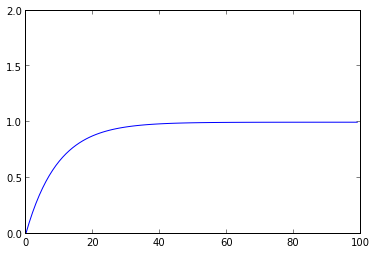
\includegraphics[width=0.33\columnwidth]{./figures/hands-on12/fig-simpleon.png}
    \caption{Expression of gene $Y$ after induction at time $t=0$.}\label{fig:simpleon}
\end{figure}
%
Your output should look like Fig.~\ref{fig:simpleon}. Notice that $Y$ reaches a steady state, $Y_{st} = \beta/\alpha$.  Take a few minutes to re-run the above code with different values of $\alpha$ and $\beta$ to understand how these two parameters interact.


Now let's put the regulation of $Y$ under the control of an external signal, $X$. When $X$ reaches a threshold $k_x$, $Y$ is transcribed. When $X$ is under this threshold, transcription of $Y$ ceases. We will make $X$ a pulse like signal, so let's write a function to generate pulses:
%
\begin{python}
def pulse(ontime, offtime,  ntimes=100, onval=1):
    signal = np.zeros(ntimes)
    signal[ontime:offtime] = onval
    return signal
\end{python}
%
And use the pulse function as follows:
%
xs = pulse(20, 80, 120)
plot(xs)
ylim(0,2)
%
Now let's update our simple simulation so $Y$ responds to $X$:
%
\begin{python}
xs = pulse(20,80,120)
alpha, beta = 0.1, 0.1
kx = 0.5
ynow = 0
ys = []
for x in xs:
    tbeta = 0
    if x > kx:
        tbeta = beta
    ynew = update(ynow, alpha, tbeta)
    ys.append(ynew)
    ynow = ynew

p1, = plot(xs)
p2, = plot(ys)
legend([p1,p2],["X","Y"])
xlabel("time")
ylim(0,2)
\end{python}
%
\begin{figure}[!ht]
    \centering
    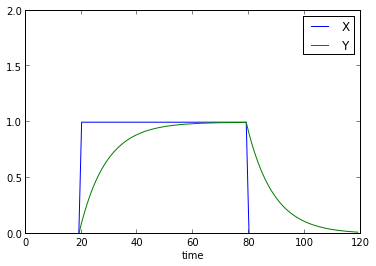
\includegraphics[width=0.33\columnwidth]{./figures/hands-on12/fig-pulse.png}
    \caption{Expression of gene $Y$ under control of signal $X$.}\label{fig:pulse}
\end{figure}
%
And now let's wrap this logic up into a simple function:
%
\begin{python}
def simplereg(xs, alpha, beta, kx, yinit=0):
    ynow = yinit
    ys = []
    for x in xs:
        talpha = alpha
        tbeta = 0
        if x > kx:
            tbeta = beta
        ynew = update(ynow, talpha, tbeta)
        ys.append(ynew)
        ynow = ynew
    return ys

\end{python}
%
We can then call this function as:
%
\begin{python}
xs = pulse(20,80,120)
ys = simplereg(xs, 0.1, 0.1, 0.5)
p1, = plot(xs)
p2, = plot(ys)
legend([p1,p2],["X","Y"])
xlabel("time")
ylim(0,2)
\end{python}
This should generate a figure identical to our previous one.

\section{Autoregulation}

Now that we've got a simple simulation working, let's get a little fancier. We'll implement a model where $Y$ negatively regulates its own transcript levels. This time we'll dive right into writing a simle function to represent   autoregulation:
%
\begin{python}
def autoreg(xs, alpha, beta, kx, alphaneg, ky, yinit=0):
    ynow = yinit
    ys = []
    for x in xs:
        talpha = alpha
        tbeta = 0
        if x > kx:
            tbeta = beta
        if ynow > ky:
            talpha = alphaneg
        ynew = update(ynow, talpha, tbeta)
        ys.append(ynew)
        ynow = ynew
    return ys
\end{python}
%
This function is almost identical to our simple regulation case, except now we check to see if $Y$ is above it's own threshold for autoregulation. If so we increase the rate of decay. We can put this |autoreg| function to work as so:
%
\begin{python}
xs = pulse(20,80,120)
ys = simplereg(xs, 0.1, 0.1, 0.5)
yneg = autoreg(xs, 0.1, 0.1, 0.5, 0.2, 0.25)

p1, = plot(xs)
p2, = plot(ys)
p3, = plot(yneg)
legend([p1,p2,p3],["$X$","$Y$","$Y_{neg}$"])
xlabel("time")
ylim(0,2)
\end{python}

We see that with negative autoregulation, $Y$ comes to a lower steady state, but also that it reaches steady state quicker than in the simple on case. It is typical to refer to the response time of a systems as the time it takes to reach one-half it's steady state value.  As we discussed in the lecture, this time is purely a function of the degradation rate, $T_{1/2} = \log(2)/\alpha$.

Negative autoregulation, when coupled with a higher rate of transcription, can be used to reach a similar steady state more quickly as shown below:
%
\begin{python}
xs = pulse(20,80,120)
ys = simplereg(xs, 0.1, 0.1, 0.5)
yneg = autoreg(xs, 0.1, 0.2, 0.5, 0.2, 0.25) # note change in 3rd argument (beta)

p1, = plot(xs)
p2, = plot(ys)
p3, = plot(yneg)
legend([p1,p2,p3],["$X$","$Y$","$Y_{neg}$"])
xlabel("time")
ylim(0,2)
\end{python}

We can use the very same |autoreg| function to implement positive autoregulation, as follows:
%
\begin{python}
xs = pulse(20,80,120)
ys = simplereg(xs, 0.1, 0.1, 0.5)
yneg = autoreg(xs, 0.1, 0.2, 0.5, 0.2, 0.25)
ypos = autoreg(xs, 0.1, 0.05, 0.5, 0.05, 0.25) # note change in 3rd and 5th args

p1, = plot(xs, lw=0.5)
p2, = plot(ys, lw=2)
p3, = plot(yneg, lw=2, ls='dashed')
p4, = plot(ypos, lw=2, ls='dashed')

legend([p1,p2,p3,p4],["$X$","$Y$","$Y_{neg}$","$Y_{pos}$"])
xlabel("time")
ylim(0,2)
\end{python}
%
\begin{figure}[!ht]
    \centering
    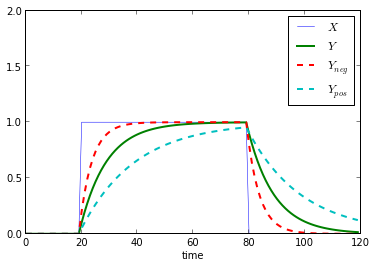
\includegraphics[width=0.33\columnwidth]{./figures/hands-on12/fig-autoreg.png}
    \caption{Contrasting simple regulation, negative autoregulation, and positive autoregulation.}\label{fig:autoreg}
\end{figure}


\section{Feed-forward Loops}

Let's add another gene, $Z$, to our network. We'll start by examing the behavior of a type of network topology (motif) called a `feed-forward loop' (FFL).


\subsection{Coherent FFLs}
The first FFL we'll examine is a `coherent FFL' -- coherent because both the short-arm (directly from $X$ to $Z$) and long-arms of the loop (with $Y$ as an intermediate) have the same effect on $Z$. In this first example, we will implement a coherent FFL with AND logic.

\begin{figure}[!ht]
\centering
\begin{tikzpicture}[node distance=2cm, auto,>=triangle 45]
  \node (X) {$X$};
  \node [right of=X] (Y) {$Y$};
  \node [right of=Y] (Z) {$Z$};
  \draw[->] (X) --  (Y);
  \draw[->] (Y) -- (Z);
  \draw[->] (X) to [bend right=30] (Z);
\end{tikzpicture}
\caption{A coherent FFL.}
\end{figure}
%
\begin{python}
def coh_ffl_and(xs, yalpha=0.1, ybeta=0.1, kxy=0.5, zalpha=0.1, zbeta=0.1, kxz=0.5, kyz=0.5):
    ynow = 0
    ys = []
    znow = 0
    zs = []
    for x in xs:
        yb = 0
        if x > kxy:
            yb = ybeta
        ynew = update(ynow, yalpha, yb)
        ys.append(ynew)

        zb = 0
        if (x > kxz) and (ynow > kyz):
            zb = zbeta
        znew = update(znow, zalpha, zb)
        zs.append(znew)

        ynow = ynew
        znow = znew
    return ys, zs
\end{python}
%
And we'll test our function with the following code:
%
\begin{python}
xs = pulse(10,15,120) + pulse(40,100,120)
ys, zs = coh_ffl_and(xs, kyz=0.5)

p1, = plot(xs)
p2, = plot(ys)
p3, = plot(zs)
legend([p1,p2,p3,p4],["$X$","$Y$","$Z$"])
xlabel("time")
ylim(0,2)
\end{python}
%
In the example above, our $X$ signal represents two pulses -- a short pulse starting at time point 10, and a more sustained pulse at time point 40. As suggested by Shen-Orr et al., and illustrated in Fig.~\ref{fig:cohffland}, the coherent FFL motif with AND logic can act as a type of sign-sensitive filter.  $Z$ doesn't turn on until $Y$ reaches a critical threshold, but both $Y$ and $Z$ turn off simultaneously.
%
\begin{figure}[!ht]
    \centering
    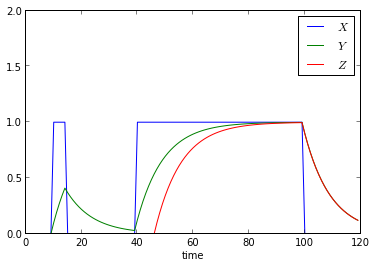
\includegraphics[width=0.33\columnwidth]{./figures/hands-on12/fig-cohffland.png}
    \caption{Behavior of a coherent FFL with AND logic at $Z$.}\label{fig:cohffland}
\end{figure}


Now let's add some random noise to our input signal, $X$.
%
\begin{python}
nxs = xs + np.random.rayleigh(0.5,size=len(xs)) # add some random noise to the signal
nxs = abs(nxs - 0.5)
plot(nxs);
\end{python}
%
Let's see how the noise effects the network:
%
\begin{python}
ys, zs = coh_ffl_and(nxs, kyz=0.5)

p1, = plot(nxs)
p2, = plot(ys)
p3, = plot(zs)
legend([p1,p2,p3,p4],["$X$","$Y$","$Z$"])
xlabel("time")
ylim(0,2)
\end{python}
%
As shown in Fig.~\ref{fig:noisyffl}, $Z$ is effectively buffered from the noise.
%
\begin{figure}[!ht]
    \centering
    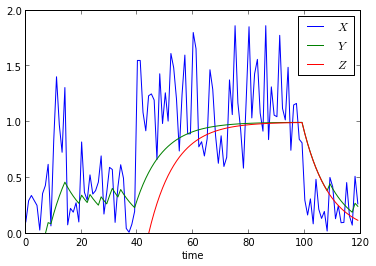
\includegraphics[width=0.33\columnwidth]{./figures/hands-on12/fig-noisyffl.png}
    \caption{Behavior of a coherent FFL with AND logic at $Z$, in response to a noisy input signal $X$.}\label{fig:noisyffl}
\end{figure}

\medskip
\begin{assignment}
Write an Python function that generates a coherent FFL with OR logic at $Z$ (i.e. $Z$ is on if either $X$ or $Y$ are above their respective thresholds), and illustrate this network motif for a variety of parameter settings.  How does the behavior of the coherent FFL with OR logic differ from the similar topology with AND logic?
\end{assignment}


\subsection{Incoherent FFLs}

Now we'll examine the behavior of an incoherent FFL, as illustrated in the figure below. As before, $X$ is an activator of both $Y$ and $Z$, but now $Y$ represses $Z$.

\begin{figure}[!ht]
\centering
\begin{tikzpicture}[node distance=2cm, auto,>=triangle 45]
  \node (X) {$X$};
  \node [right of=X] (Y) {$Y$};
  \node [right of=Y] (Z) {$Z$};
  \draw[->] (X) --  (Y);
  \draw[-|] (Y) -- (Z);
  \draw[->] (X) to [bend right=30] (Z);
\end{tikzpicture}
\caption{An incoherent FFL.}
\end{figure}

\begin{python}
def incoh_ffl_and(xs, yalpha=0.1, ybeta=0.1, kxy=0.5, zalpha=0.1, zbeta=0.1, kxz=0.5, kyz=0.5):
    ynow = 0
    ys = []
    znow = 0
    zs = []
    for x in xs:
        yb = 0
        if x > kxy:
            yb = ybeta
        ynew = update(ynow, yalpha, yb)
        ys.append(ynew)

        zb = 0
        if (x > kxz) and (ynow < kyz):
            zb = zbeta
        znew = update(znow, zalpha, zb)
        zs.append(znew)

        ynow = ynew
        znow = znew
    return ys, zs
\end{python}
%
And we'll test our new function as follows:
%
\begin{python}
xs = pulse(10,40,180) + pulse(70,140,180)
ys, zs = incoh_ffl_and(xs, kyz=0.75)

p1, = plot(xs)
p2, = plot(ys)
p3, = plot(zs)

legend([p1,p2,p3,p4],["$X$","$Y$","$Z$"])
xlabel("time")
ylim(0,2)
\end{python}
%
This produces Fig.~\ref{fig:incohfll}.  Incoherent FFLs are capable of producing pulsatile behaviors. Notice how the length of the pulses in $Z$ are insensitive to longer input signals $X$ (they are however sensitive to very short pulses in $X$).
%
\begin{figure}[!ht]
    \centering
    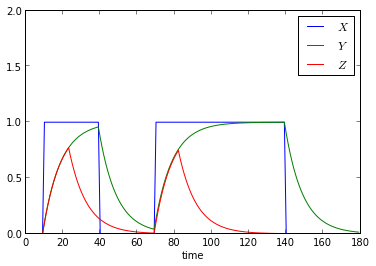
\includegraphics[width=0.33\columnwidth]{./figures/hands-on12/fig-incohffl.png}
    \caption{Behavior of an incoherent FFL with AND logic at $Z$.}\label{fig:incohfll}
\end{figure}

\section{Repressilator}

Elowitz and Liebler (Nature, 403(6767):335-8) proposed that a synthetic network motif that they called the `repressilator' could generate sustained oscillatory behavior. This network motif consists of three genes that mutually repressor each other, as illustrated in Fig.~\ref{fig:repressilator}.
\begin{figure}[!ht]
\centering
\begin{tikzpicture}[node distance=2cm, auto,>=triangle 45]
  \node (X) {$X$};
  \node [right of=X] (Y) {$Y$};
  \node [right of=Y] (Z) {$Z$};
  \draw[-|] (X) --  (Y);
  \draw[-|] (Y) -- (Z);
  \draw[-|] (Z) to [bend right=30] (X);
\end{tikzpicture}
\caption{The repressilator network motif.}\label{fig:repressilator}
\end{figure}
%
Let's implement the repressilator motif as a Python function:
\begin{python}
def repressilator(xalpha, xbeta, yalpha, ybeta, zalpha, zbeta, kxy=0.5, kyz=0.5, kzx=0.5, xinit=1, yinit=1, zinit=1, nticks=500):
    xnow = xinit
    xs = []
    ynow = yinit
    ys = []
    znow = zinit
    zs = []

    for i in range(nticks):
        if xnow < kxy:
            ya, yb = yalpha, ybeta
        else:
            ya, yb = yalpha, 0
        ynew = update(ynow, ya, yb)
        ys.append(ynew)

        if ynow < kyz:
            za, zb = zalpha, zbeta
        else:
            za, zb = zalpha, 0
        znew = update(znow, za, zb)
        zs.append(znew)

        if znow < kzx:
            xa, xb = xalpha, xbeta
        else:
            xa, xb = xalpha, 0
        xnew = update(xnow, xa, xb)
        xs.append(xnew)

        ynow = ynew
        znow = znew
        xnow = xnew

    return xs, ys, zs
\end{python}
%
And we can test it as we've done previously:
\begin{python}
xs,ys,zs = repressilator(0.1,1, 0.1,2, 0.1,2)
p1, = plot(xs)
p2, = plot(ys)
p3, = plot(zs)

legend([p1,p2,p3,],["$X$","$Y$","$Z$"])
xlabel("time")
\end{python}
%
\begin{figure}[!ht]
    \centering
    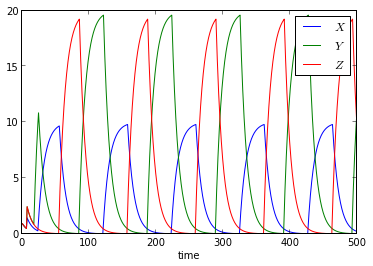
\includegraphics[width=0.33\columnwidth]{./figures/hands-on12/fig-repressilator.png}
    \caption{Behavior of the repressilator network motif.}\label{fig:repressdynamics}
\end{figure}



\medskip
\begin{assignment}
Spend some time exploring the parameter space of the repressilator motif.  Under what conditions does the system \emph{NOT} oscillate?  What parameters can you change to get longer oscillations (i.e. longer intervals between peak values for a given gene)?  Generate graphs to illustrate the cases above.
\end{assignment}